%%%administrators guide for libpniutils

\documentclass[a4paper,twoside]{book}
\usepackage{a4wide,amsmath,graphics}
\usepackage{listings}
\author{Eugen Wintersberger}
\title{{\Huge libpniutils\\ Users guide}}

%%setup the listings package
\lstset{language=C++}
\lstdefinestyle{numbers}{numbers=left,stepnumber=1,numberstyle=\small}
\lstset{style=numbers}
\lstset{captionpos=b,frame=lines,float=tb}
\lstset{floatplacement=tb}

\begin{document}
\maketitle
\tableofcontents

\chapter{Introduction}\label{chapter:introduction}
%%%a general introduction into libpnicore


%%%============================================================================
\section{The PNI library stack}

%%%----------------------------------------------------------------------------
\begin{figure}[tb]
\centering
\resizebox{0.8\linewidth}{!}{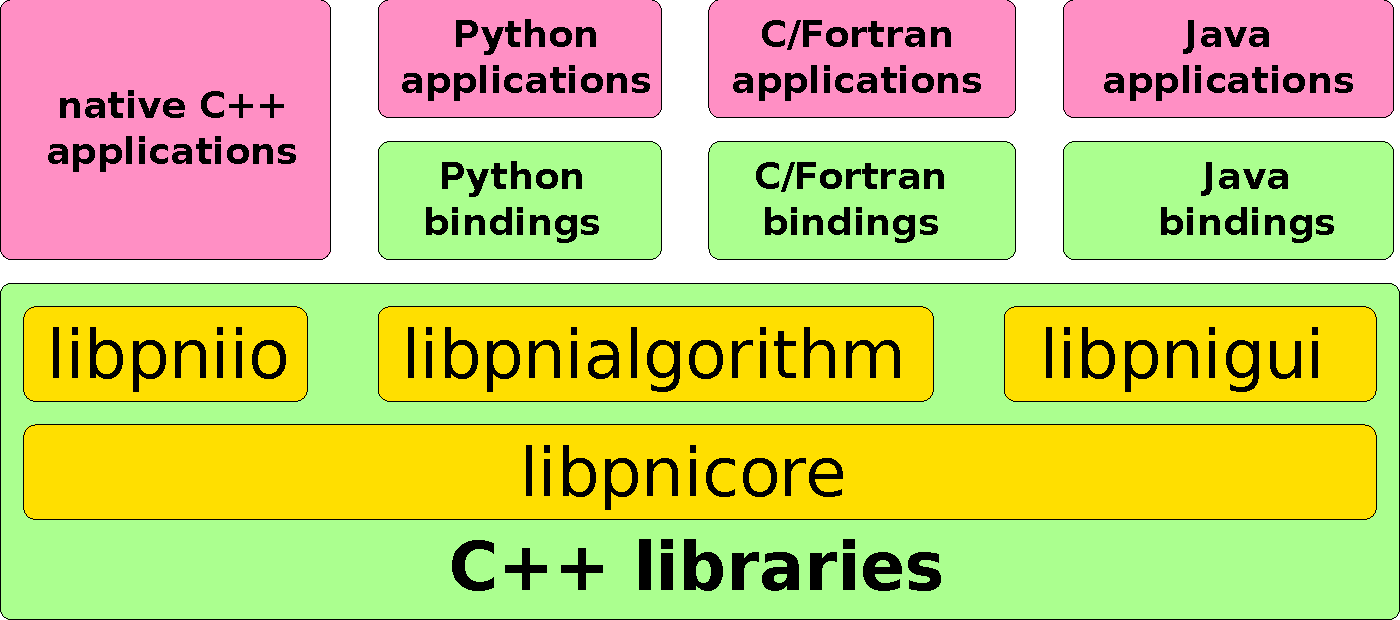
\includegraphics{pics/pni-cpp-libraries.pdf}}
\caption{{\small\label{fig:intro:libstack} 
The PNI library stack is a collection of C++ libraries developed with the
intention to simplify the process of writing application in the PNI field.
\libpnicore , the library described in this manual is the foundation of this
stack. It provides all the basic data structures and facilities used by all
other libraries.}}
\end{figure}
%%%----------------------------------------------------------------------------

\libpnicore\ is one of the PNI libraries developed within the framework of the
HDRI project. As shown in Fig.~\ref{fig:intro:libstack} \libpnicore\ it is the
foundation for all libraries in the stack. None of them can be used
without it. 
\libpnicore\ provides the basic data structures used by all other PNI libraries. 
This includes
\begin{itemize}
    \item well defined data types
    \item multidimensional arrays
    \item configuration facilities 
    \item type erasures.
\end{itemize}



%%%============================================================================
\section{How to read this manual}

For a new user the best way to read this manual is from beginning to the end.
One may can omit the next chapter about installation of the library if this is
done by your local system administrator. In any case, a new user should should
definitely start with Chapter~\ref{chapter:using_library}.

The library makes heavy use of C++11 features. There are plenty of websites on
the internet explaining those new features. For an experienced C++ programmer 
the Wiki site\cite{web:cpp11wiki} describing the new features for C++11 might be
enough. However, new users with less experience in modern C++ may should
purchase one of the excellent books available on this language.

A reader already familiar with \libpnicore\ may uses this guide as a short
reference to the most important features. In any case, more detailed information
about each class can be found in the API documentation.





\chapter{Basic concepts}\label{chapter:basics}
%%%basic considerations about the PNI utilities library

\chapter{Using the library}\label{chapter:usage}
\input{tex/usage.tex}

\chapter{Data in memory}\label{chapter:data_in_memory}
%%%documentation for data objects in memory

One of the primary obstacles of this library is to provide the user with a 
couple of easy to use objects to handle data in its program. 
Thus, libpniutils provides two fundamental class templates
\begin{itemize}
  \item {\tt Scalar<T>} describing a single scalar
  \item {\tt Array<T>} describing a multidimensional array.
\end{itemize}
These templates should be used along with the native data types defined by the 
library ans shown in \ref{tab:datatypes} and defined in the header file
{\tt PNITypes.hpp}.
Along with the data values these objects provide additional information 
about themself. These information is
\begin{description}
\item[name] the name of the object
\item[description] a string with a short description about the object
\item[unit] a string with a physical unit which can be usefull if data 
            should be plotted.
\end{description} 
With this meta-data a single datum is sufficiently described. 

\begin{table}[tb]
\begin{tabular}{l|c|c|l}
\hline
Name & C++ type & size in bits & description \\
\hline
{\tt UInt8} & {\tt unsigned char}& $8$ & $8$Bit unsigned integer\\
{\tt Int8}  & {\tt char } & $8$ & $8$Bit signed integer \\
{\tt UInt16} & {\tt unsigned short} &$16$ & $16$Bit unsigned integer \\
{\tt Int16} & {\tt short} & $16$ & $16$Bit signed integer \\
{\tt UInt32} & {\tt unsigned int} & $32$ & $32$Bit unsigned integer\\
{\tt Int32} & {\tt int} & $32$ & $32$Bit signed integer \\
{\tt UInt64} & {\tt unsigned long} & $64$ & $64$Bit unsigned integer\\
{\tt Int64} & {\tt long} & $64$ & $64$Bit singed integer \\ 
\hline
{\tt Float32} & {\tt float} & $32$ & $32$Bit IEEE floating point number \\
{\tt Float64} & {\tt double} & $64$ & $64$Bit IEEE floating point number \\
{\tt Float128} & {\tt long double} & $128$ & $128$Bit IEEE floating point number
\\
\hline
{\tt Complex32} & {\tt std::complex<float>} & - & $2\times32$Bit IEEE complex number \\
{\tt Complex64} & {\tt std::complex<double>} & - & $2\times64$Bit IEEE complex
number \\
{\tt Complex128} & {\tt std::complex<long double>} & - & $2\times128$Bit IEEE
complex number \\
\hline
\end{tabular}
\caption{{\small \label{tab:datatypes} Native data types of well defined size.
These data types are defined in the header file {\tt PNITypes.hpp} and should 
be used throughout a program instead of the standard data types provided by 
your C++ compiler. The reason is that the size of the types provided by your 
compiler differ from those given here depending on your hardware platform.}}
\end{table}

The two templates mentioned above will be described first in this chapter.
The last chapter deals with the class hierarchy the two templates belong to.

\section{The {\tt Scalar<T>} template}

This is most probably the simplest template of the high level data objects. 
Basically it holds a single numerical value along with the additional 
information mentioned above. 
On the first glimpse this template might look slightly bloated. Why an 
entire template just for a single number. The reason is the additional
meta-information mentioned above. An object instantiated from the template 
behaves nearly like a common C++ native variable. The fundamental 
arithmetic operators are overloaded and thus these objects can be used 
like native variables. 
However, 

\subsection{Instantiation of a {\tt Scalar<T>} template}

Besides the default and a copy constructor, the {\tt Scalar<T>} template 
provides a whole bunch of constructors to configure an object right at the 
moment of its instantitation.
So using the standard default and copy constructor is fairly simple
\begin{verbatim}
//default constructor
Scalar<UInt16> SCA1;
//here comes some configuration code for SCA1

//create a second SCA object from SCA1
Scalar<UInt16> SCA2(SCA1);
\end{verbatim} 
The remaining constructors can be divided into two groups: those setting 
and initial data value to the object and those who are not. 
The former one can be used as shown here
\begin{verbatim}
//motor with initial value
Scalar<Float32> motor1(14.34);

//setting value, name, and unit
Scalar<Float32> motor2(45.21,"omega","degree");

//setting value, name, unit, and description
Scalar<Float32> motor3(90.32,"theta","degree","detector angle");
\end{verbatim}
while the later ones are simply
\begin{verbatim}
//setting value, name, and unit
Scalar<Float32> motor2("omega","degree");

//setting value, name, unit, and description
Scalar<Float32> motor3("theta","degree","detector angle");
\end{verbatim}
All information that can be passed to the constructor can be changed 
and accessed after object instantiation via the apropriate methods as 
will be shown in the next section.

\subsection{Accessing {\tt Scalar<T>} object information and data}
After an instance of {\tt Scalar<T>} has been created we can use methods 
to configure this object. In this next code snipped we will use 
the default constructor for instantiation and afterwards 
configure the object using the appropriate methods
\begin{verbatim}
Scalar<UInt32> SCA;     //class instantiation
SCA.setName("SCA1");    //set the name of the object
SCA.setUnit("cps");     //set the unit to (cps)
SCA.setDescription("first SCA in the rack");  //set the description

SCA.setValue(30392);   //setting a data value 
\end{verbatim}
As shown already in the previous section we could have achieved the same 
object using an single constructor call. However, in some cases it is 
not possible to know everything about an object at the time it is 
created.
We can obtain all the information and data from an object using the 
corresponding {\tt get}-methods (as you may have already expected)
\begin{verbatim}
String name = SCA.getName();         //obtain the name of the object
String unit = SCA.getUnit();         //its unit
String desc = SCA.getDescription();  //its description
UInt32 data = SCA.getValue();        //and finaly its data value
\end{verbatim}
In particular using {\tt getValue()} nad {\tt setValue()} for reading from
and and writing data to the object feels quite unnatural. In the next section
a method for accessing a {\tt Scalar<T>}s data using the assignment operator 
will be introduced which makes such an object fell much more like a native 
type variable.

\subsection{Assignment of a {\tt Scalar<T>} template and conversion operator}

While object creation is a rather simple task assignment is not that
easy\footnote{ For those who are not that familiar with C++: If you create an
object from another you can always assume that you start with a new object. 
If you assign an object to an other you have to take measures that the
assignment leads to an valid result.}.
Assignment means that the values of an already existing {\tt Scalar<T>} object 
will be assigned to an other object of that type. In addition and particularlly
useful for this special type of object is the assigment of a native variable 
to a {\tt Scalar<T>} object.
From this we get four possible cases which must be handled by the assignment
operator
\begin{enumerate}
  \item assign a {\tt Scalar<T>} to an other {\tt Scalar<T> } - this is the
  trivial case
  \item assign a varible of type {\tt T} to an instance {\tt Scalar<T>}
  \item assign a {\tt Scalar<U>} to an instance of {\tt Scalar<T>} where {\tt U}
  and {\tt T} are different native types
  \item and finally assign a variable of native type {\tt U} to a {\tt
  Scalar<T>} object where {\tt T} and {\tt U} denote differnt native types.
\end{enumerate}
The first two cases are trivial and are fully supported as shown in this 
next code snippet
\begin{verbatim}
Scalar<UInt32> SCA1;
Scalar<UInt32> SCA2;
Scalar<UInt32> SCA;
UInt32 data = 101983;

//assign here the SCA1 or SCA2 to SCA
if(...){ 
    SCA = SCA1;
}else{
    SCA = SCA2;
}

//set the value of SCA using the assignment operator
SCA = data;
\end{verbatim}
There is a small difference in the usage of the assignment operator in this 
way. In the first case where for instance {\tt SCA = SCA1;} {\tt SCA} not 
only takes the value of {\tt SCA1} it also obtains its name, unit, and 
description. This is what one would expect from an assignment operator 
in C++. In the latter case {\tt SCA = data} only the value of {\tt SCA} is set
to that of {\tt data}. 

The other two situations as mentioned above where the rhs of the assignment 
operator is based on a different native type is a bit more complicated. 
In both cases the value of the object on the lhs of the assignment operator 
must take a value of a different native type. It is quite clear that this is 
not always possible without complications. If you assign variables of 
incompatible native types (for instance if you try to assigne a singned integer
to an variable of an unsiged type) in C++ you usually get neither an error
message or an exception. However, for the {\tt Scalar<T>} object this is the 
case. Thus not all combinations of assignments are allowed if the fundamental 
data types on the lhs of the assignment operator differ from those of the 
rhs.
There are two basic rules
\begin{enumerate}
  \item you cannot assign a float or complex to an integer scalar - this will
  throw an {\tt TypeError} exception
  \item you cannot assign a complex type to a float type - this will throw
  an {\tt TypeError} exception.
\end{enumerate}
All other assignments are permitted. However, the library checks out of 
bound situations where the assigned value exceeds the bounds of the 
type it should be assigned to. In such cases a {\tt RangeError} exception 
is thrown. 

Until now only the case where the template class {\tt Scalar<T>} resided on 
the lhs of an assignment. Since the conversion operator is overloaded 
for {\tt Scalar<T>} you can assign the value of an instance of {\tt Scalar<T>}
directly to a native variable using the assignment operator. 
Such an expression would look like this:
\begin{verbatim}
Scalar<Float32> s(100.2);
Float32 t = s;
\end{verbatim}
There is one limittation with this approach: it does not work for 
complex numbers. 
\begin{center}
{\HUGE MAKE A REMARK HERE THAT YOU CANNOT DO THIS WITH COMPLEX NUMBERS!}
\end{center}
The conversion operator is also responsible that there is 
no need for overloading order operators like {\tt <} or {\tt >}. If 
we use them the compiler uses the converion operator to access the value of 
a {\tt Scalar<T>} object and thus can use the native order operators provided 
by C++.  

\subsection{Comparison of scalars}

As already mentioned scalar objects should behave nearly like native C++
variables - this should be valid also for the operators {\tt ==} and {\tt !=}.
In general we have to discuss two situations
\begin{enumerate}
  \item comparsion between two objects of type {\tt Scalar<T>} and {\tt
  Scalar<U>} where {\tt U} and {\tt T} denote not necessarily the same 
  native data type
  \item and comparison between an object of type {\tt Scalar<T> } and a 
  native variable of type {\tt U} where {\tt U} and {\tt T} can denote
  different types.
\end{enumerate}
 The question is which data of a {\tt Scalar<T>} object should be compared.
In the latter case the situation is simple: we can only compare the value of the 
object with the value of the native variable. 
For the former situation one has to think a bit more. It makes no sense to
check the name or the description of an object for equality. 
However, it makes sense to compare units. In this case we avoid that 
a user    


\subsection{Ordering operators}

Ordering operators only can check the value of a scalar object.   


\subsection{Arithemtic operations}
Both the binary as well as the unary arithmetic operations are overloaded 
for the {\tt Scalar<T>} template. Like the assignment operator the arithmetic
operators take care about type problems. Usually you would not recognize
problems with types during arithmetic operations. However there are some 
and they should be mentioned here in order to inform you about when and why 
exceptions are thrown. The situation is a bit different for binary and unary 
operators thats why they are handled in different sections.

\subsubsection{The unary arithmetic operators}
The following unary operators are overloaded: {\tt +=}, {\tt -=}, {\tt *=}, and
{\tt /=} for the following situations
\begin{description}
\item[{\tt Scalar<T> ?= Scalar<T>}] the trivial case 
\item[{\tt Scalar<T> ?= T}] trivial too because equal type
\item[{\tt Scalar<T> ?= U}] have to check types
\item[{\tt Scalar<T> ?= Scalar<U>}] have to check types
\end{description}
here {\tt ?=} denotes one of the above unary operators. The first two versions
of an operator are trivial since lhs and rhs have the same fundamtal data
type. The last to need some special handling to avoid overflow problems or 
to avoid operations which would make no sense (this is simply because the 
type of the lhs object is already determined - this situaetion is different 
for binary operators).
We can deduce the following general rules
\begin{enumerate}
  \item operations with complex types are only supported if lhs and rhs are
  complex - otherwise a {\tt TypeError} exception will be thrown
  \item if the lhs is an integer the rhs must not be of a float type
  \item integer divisions are only supported if the value of the lhs is a 
        multiple integer of the rhs - otherwise a {\tt RangeError} will be 
        thrown
  \item if the lhs is an unsigned integer the result 
\end{enumerate}


\subsubsection{The binary arithmetic operators}

The following binary operators are overloaded for all data types: $+$, $-$, $*$,
and $/$. These operators are implemented as templates using a special 
{\tt ResultTypeTrait} template to determine the result type of an operation. 
Thus, we do not have to perform any checking of the arguments 
data types. Both input arguments are first transformed to the result type 
before the operation is performed. 
The binary operators create a third intermediate result type of the 
appropriate result type which holds the result of the operation and which 
will be returned to the caller of the operator. There the result scalar of the 
operation is assigned to the proposed scalar type. If the automatically 
derived result type and the proposed type do not match an exception will be
thrown. 

\subsection{A full example}

\section{The {\tt Array<T>} template}

\subsection{Instantiation of a {\tt Array<T>} template}

\subsection{Assignment of a {\tt Array<T>} template}

\subsection{Arithmetic operations}

\subsection{Array selections}

\subsection{A full example}

\chapter{Data I/O}\label{chapter:io}

\chapter{Exceptions}\label{chapter:exceptions}

\appendix
\chapter{Low level objects}
%%%some text about buffers
\section{Buffer objects}
Buffers play an important role within the library. Usually you do not need 
to care about them. However, for library developers it is important 
to know how they work.

A buffer represents a number of elements of a particular size linearly 
stored in memory. Thus is behaves somehow like an array or one of the 
container templates provided by the STL. However, it follows its own 
allocation and reallocation policy which will be described here in more detail.  

The aim of a buffer is to allocate memory for a number of objects of equal 
size. Therefore, the amount of memory allocated depends on two parameters
\begin{enumerate}
  \item the {\em element size } which is the size of each element in bytes
  \item the {\em size } of the buffer which is the number of elements in the
  buffer.
\end{enumerate}
The total amount of memory which must be allocated to hold this data is 
than given with
\begin{align}
n_{\mathrm{tot}} = \mathrm{element size}\times\mathrm{size}.
\end{align}

All buffers should be derived from the {\tt BufferObject} base class which 
holds the minimal interface each buffer object should implement. 
The base class itself only provides simple managment functions for the
size of the allocated memory. However, it already implies some of the 
policies that each buffer object should follow. 
There are three situations a buffer object must face
\begin{enumerate}
  \item instantiation
  \item allocation
  \item assignment
  \item reallocation
\end{enumerate} 

\subsection{Instantiation of buffer objects}

Buffers allow the allocation of memory to be posponed to a later point in 
time after their creation. This of coarse has some implications. 
It is necessary to keep track of a buffers state in every method that 
can effect the allocated memory. 




The template {\tt Buffer<T>} is a concrete implementation 



\end{document}